\documentclass[a4paper]{article}
\usepackage{graphicx}
\usepackage[cm]{fullpage}
\usepackage{bm}
\usepackage{listings}
\usepackage{color}
\usepackage{amsmath}
\usepackage{amsfonts}
\usepackage{hyperref}
\hypersetup{
    colorlinks,
    citecolor=black,
    filecolor=black,
    linkcolor=black,
    urlcolor=black
}
\lstset{ 
  language=Python,
  backgroundcolor=\color{white},   % choose the background color; you must add \usepackage{color} or \usepackage{xcolor}; should come as last argument
  basicstyle=\footnotesize,        % the size of the fonts that are used for the code
  breakatwhitespace=false,         % sets if automatic breaks should only happen at whitespace
  breaklines=true,                 % sets automatic line breaking
  captionpos=b,                    % sets the caption-position to bottom
  frame=single,                    % adds a frame around the code
  keepspaces=true,                 % keeps spaces in text, useful for keeping indentation of code (possibly needs columns=flexible)
  keywordstyle=\color{blue},       % keyword style
}



\title{The Finite Element Method in Geodynamics}

\author{C. Thieulot}

\begin{document}

\maketitle

\tableofcontents

\newpage
%%%%%%%%%%%%%%%%%%%%%%
\section{Introduction}

practical hands-on approach

as little as possible jargon

no mathematical proof

no optimised codes (readability over efficiency). avoiding as much as possible to have to look elsewhere.
very sequential, so unavoidable repetitions (jacobian, shape functions)

FE is one of several methods.

\subsection{Acknowledgments}

Jean Braun, Philippe Fullsack, Arie van den Berg.
Lukas van de Wiel. Robert Myhill.
Menno, Anne
Too many BSc and MSc students to name indivisually, although Job Mos did produce the
very first version of fieldstone as part of his MSc thesis.
The ASPECT team in general and Wolfgang Bangerth in particular.

%--------------------------------
\subsection{Essential literature}

\begin{center}
a)\includegraphics[height=4cm]{images/literature/gerya_book}
b)\includegraphics[height=4cm]{images/literature/tackley_book}
c)\includegraphics[height=4cm]{images/literature/donea_huerta_book}
d)\includegraphics[height=4cm]{images/literature/bercovici_book}
e)\includegraphics[height=4cm]{images/literature/sto_book}\\
%a) \url{https://doi.org/10.1017/CBO9780511809101}
%b) \url{https://doi.org/10.1017/CBO9780511780820}
%c) \url{https://www.wiley.com/en-us/Finite+Element+Methods+for+Flow+Problems-p-9780471496663}
%d) \url{https://www.elsevier.com/books/treatise-on-geophysics-volume-7/bercovici/978-0-444-51935-1}
\end{center}

%---------------------------------------
\subsection{Installation}

\begin{verbatim}
python3.6 -m pip install --user numpy scipy matplotlib
\end{verbatim}



\newpage
%%%%%%%%%%%%%%%%%%%%%%
\section{The physical equations of Fluid Dynamics}

[from aspect manual]
We focus on the system of equations in a $d=2$- or $d=3$-dimensional
domain $\Omega$ that describes the motion of a highly viscous fluid driven
by differences in the gravitational force due to a density that depends on
the temperature. In the following, we largely follow the exposition of this
material in Schubert, Turcotte and Olson \cite{scto01}.

Specifically, we consider the following set of equations for velocity $\mathbf
u$, pressure $p$ and temperature $T$:
\begin{align}
  \label{eq:stokes-1}
  -\nabla \cdot \left[2\eta \left(\dot\varepsilon(\bm v)
                                  - \frac{1}{3}(\nabla \cdot \bm v)\mathbf 1\right)
                \right] + \nabla p &=
  \rho \bm g
  &
  & \textrm{in $\Omega$},
  \\
  \label{eq:stokes-2}
  \nabla \cdot (\rho \bm v) &= 0
  &
  & \textrm{in $\Omega$},
  \\
  \label{eq:temperature}
  \rho C_p \left(\frac{\partial T}{\partial t} + \bm v\cdot\nabla T\right)
  - \nabla\cdot k\nabla T
  &=
  \rho H
  \notag
  \\
  &\quad
  +
  2\eta
  \left(\dot\varepsilon(\bm v) - \frac{1}{3}(\nabla \cdot \bm v)\mathbf 1\right)
  :
  \left(\dot\varepsilon(\bm v) - \frac{1}{3}(\nabla \cdot \bm v)\mathbf 1\right)
  \\
  &\quad
  +\alpha T \left( \bm v \cdot \nabla p \right)
  \notag
  \\
  &\quad
  + \rho T \Delta S \left(\frac{\partial X}{\partial t} + \bm v\cdot\nabla X\right)
  &
  & \textrm{in $\Omega$},
  \notag
\end{align}
where $\dot\varepsilon(\mathbf u) = \frac{1}{2}(\nabla \mathbf u + \nabla\mathbf
u^T)$ is the symmetric gradient of the velocity (often called the
\textit{strain rate}).%

In this set of equations, \eqref{eq:stokes-1} and \eqref{eq:stokes-2}
represent the compressible Stokes equations in which $\mathbf v=\mathbf
v(\mathbf x,t)$ is the velocity field and $p=p(\mathbf x,t)$ the pressure
field. Both fields depend on space $\mathbf x$ and time $t$. Fluid flow is
driven by the gravity force that acts on the fluid and that is proportional to
both the density of the fluid and the strength of the gravitational pull.

Coupled to this Stokes system is equation \eqref{eq:temperature} for the
temperature field $T=T(\mathbf x,t)$ that contains heat conduction terms as
well as advection with the flow velocity $\mathbf v$. The right hand side
terms of this equation correspond to
\begin{itemize}
\item internal heat production for example due to radioactive decay;
\item friction heating;
\item adiabatic compression of material;
\item phase change.
\end{itemize}
The last term of the temperature equation corresponds to
the latent heat generated or consumed in the process of phase change of material. 
In what follows we will not assume that no phase change takes place so that we disregard this term 
altogether.

%---------------------------------
\subsection{the Boussinesq approximation: an Incompressible flow}

[from aspect manual]
The Boussinesq approximation assumes that the density can be
considered constant in all occurrences in the equations with the exception of
the buoyancy term on the right hand side of \eqref{eq:stokes-1}. The primary
result of this assumption is that the continuity equation \eqref{eq:stokes-2}
will now read
\[
{\bm \nabla}\cdot{\bm v} = 0
\]
This implies that the strain rate tensor is deviatoric.
Under the Boussinesq approximation, the equations are much simplified:

\begin{align}
  \label{eq:stokes-1}
  -\nabla \cdot \left[2\eta \dot\varepsilon(\bm v)
                \right] + \nabla p &=
  \rho \bm g
  &
  & \textrm{in $\Omega$},
  \\
  \label{eq:stokes-2}
  \nabla \cdot (\rho \bm v) &= 0
  &
  & \textrm{in $\Omega$},
  \\
  \label{eq:temperature}
  \rho_0 C_p \left(\frac{\partial T}{\partial t} + \bm v\cdot\nabla T\right)
  - \nabla\cdot k\nabla T
  &=
  \rho H
  &
  & \textrm{in $\Omega$}
\end{align}
Note that all terms on the rhs of the temperature equations have disappeared, with the exception 
of the source term.

These are the equations which are used and implemented in all the codes, unless otherwise
indicated.

%---------------------------------
\subsubsection{The penalty approach}

In order to impose the incompressibility constraint, two widely used procedures are available, namely the 
Lagrange multiplier method and the penalty method \cite{bathe82,hugh}. The latter is implemented in {\sc elefant}, which allows for the elimination of the pressure variable from the momentum equation (resulting in a reduction of the matrix size).%, based on a relaxation of the incompressibility constraint. 

Mathematical details on the origin and validity of the penalty approach applied to the Stokes problem can for instance be found in  \cite{cuss86}, \cite{redd82} or \cite{gunz89}.

The penalty formulation of the mass conservation equation is based on a relaxation of the incompressibility constraint and writes 
\begin{equation}
{\bm \nabla}\cdot {\bm v} + \frac{p}{\lambda} = 0 \label{penal}
\end{equation}
where $\lambda$ is the penalty parameter, that can be interpreted (and has the same dimension) as a bulk viscosity. It is 
equivalent to say that the material is weakly compressible. It can be shown that if one chooses $\lambda$ to be a 
sufficiently large number, the continuity equation $ {\bm \nabla}\cdot {\bm v} = 0$ will be approximately satisfied in the finite element solution. The value of $\lambda$ is often recommended to be 6 to 7 orders of magnitude larger than the shear viscosity \cite{dohu03,hulb79}.

%Note that Eq. (\ref{penal}) does not form the basis of the penalty method (as often implied) for the Stokes equation but is a consequence of minimising a modified functional of the problem under certain assumptions \cite{redd82}. 

Equation (\ref{penal}) can be used to eliminate the pressure in Eq. (\ref{mce2}) so that the mass and momentum conservation equations fuse to become :
\begin{equation}
{\bm \nabla}\cdot ( 2 \eta \dot\varepsilon({\bm v})) + \lambda {\bm \nabla} ({\bm \nabla }\cdot {\bm v}) = \rho {\bm g} = 0 \label{peneq}
\end{equation}

\cite{mahu78} have established the equivalence for incompressible problems between the reduced integration
of the penalty term and a mixed Finite Element approach if the pressure nodes coincide with the integration points of the reduced rule.

In the end, the elimination of the pressure unknown in the Stokes equations
replaces the original saddle-point Stokes problem \cite{begl05} by an elliptical problem, 
which leads to a symmetric positive definite (SPD) FEM matrix. 
%Such systems always admit a square root triangular matrix (the Cholesky factor, L) and can be solved, once L has been computed (Cholesky factorization), by 2 triangular matrix solves (upper and lower back-substitutions). 
This is the major benefit of the penalized approach 
over the full indefinite solver with the velocity-pressure variables. Indeed, the SPD character of the matrix lends itself 
to efficient solving stragegies and is less memory-demanding since it is sufficient to store only the upper half of the matrix including the diagonal
\cite{gova}
.
ToDo: list codes which use this approach.





\newpage
%------------------------------------------------------------------------------
\section{The Finite Element Method}

\subsection{aaa}


\subsection{Solving procedures}

\subsubsection{the whole matrix at once}

\subsubsection{the pressure Schur complement appraoch}



\newpage
%------------------------------------------------------------------------------
\section{Additional techniques}

\subsection{The method of manufactured solutions}

\subsection{Sparse storage}

\subsection{Mesh generation}

\subsection{The value of the timestep}

\subsection{Tracking materials}

\subsection{Visco-Plasticity}

\subsection{Picard and Newton}

\subsection{The choice of solvers}

\subsection{The SUPG formulation for the energy equation}

\subsection{Tracking materials and/or interfaces}

\subsection{Dealing with a free surface}









\newpage
so much to do ... 

impose bc on el matrix

Q2Q1 

Q3Q2

3D - Burstedde benchmark 

full compressible 

total energy calculations

constraints

Q1Q1-stab

non-linear rheologies (punch, two layer brick spmw16, tosn15) 

Picard vs Newton

markers

Schur complement approach

periodic boundary conditions

open boundary conditions

export to vtu 

free surface 

SUPG

produce fastest version possible for convection box

zaleski disk advection

all kinds of interesting benchmarks

Busse convection pb, compare with aspect 

cvi !!!

pure elastic 

including phase changes (w. R. Myhill)

derivatives on nodes

Nusselt

aBBT matrix as whole to solver?

discontinuous galerkin

formatting of code style

navier-stokes ? (LUKAS)

pressure smoothing

compute strainrate in middle of element or at quad point for punch?

GEO1442 code 

GEO1442 indenter setup in plane ?

in/out flow on sides for lith modelling

\noindent Problems to solve:

colorscale 

velocity arrows 

better yet simple matrix storage ?


\newpage
%%%%%%%%%%%%%%%%%%%%%%%%%%%%%%%%%%%%%%%%%%%%%%%%%%%%%%%%%%%%%%%%%%%%%%%%%%%%%%%
\section{{\tt fieldstone}: simple analytical solution}

From \cite{dohu}. In order to illustrate the behavior of selected mixed finite elements in the solution 
of stationary Stokes flow,  we consider a two-dimensional problem 
in the square domain $\Omega=[0,1]\times[0,1]$, which possesses a closed-form analytical 
solution. The problem consists of determining the velocity field ${\bm v} = (u,v)$ and the 
pressure $p$ such that 
\[
-\nu \Delta {\bm v} + {\bm \nabla} p = {\bm b}  \quad\quad {\rm in} \; \Omega
\]
\[
{\bm \nabla} \cdot {\bm v} = 0 \quad\quad {\rm in} \; \Omega
\]
\[
{\bm v}={\bm 0} \quad\quad {\rm on} \; \Gamma
\]
where the fluid viscosity is taken as $\nu=1$. The components of the body force ${\bm b}$ are prescribed as 
\begin{eqnarray}
b_x &=& (12 - 24y) x^4 + (-24 + 48y) x^3 + (-48y + 72y^2 - 48 y^3 + 12) x^2 \nonumber\\
    && + (-2 + 24y -72y^2+48y^3)x + 1-4y + 12y^2-8y^3 \nonumber\\ 
b_y &=& (8 - 48y + 48 y^2) x^3 + (-12 + 72y - 72y^2) x^2  \nonumber\\
    && + (4 - 24y + 48y^2 - 48y^3 + 24y^4) x - 12y^2 + 24y^3 - 12y^4  \nonumber
\end{eqnarray}
With this prescribed body force, the exact solution is 
\begin{eqnarray}
u(x,y) &=& x^2(1- x)^2 (2y - 6y^2 + 4y^3)  \nonumber\\
v(x,y) &=& -y^2 (1 - y)^2 (2x - 6x^2 + 4x^3) \nonumber\\
p(x,y) &=& x(1 -x)- 1/6 \nonumber 
\end{eqnarray}
Note that the pressure obeys $\int_{\Omega} p \; d\Omega = 0$

\fbox{
\parbox{10cm}{{\bf features}
\begin{itemize}
\item $Q_1\times P_0$ element
\item incompressible flow
\item penalty formulation
\item Dirichlet boundary conditions (no-slip)
\item direct solver
\item isothermal
\item isoviscous
\item analytical solution
\end{itemize}
}}

\includegraphics[width=16cm]{python_codes/fieldstone/solution.pdf}

\begin{center}
\includegraphics[width=12cm]{python_codes/fieldstone/errors.pdf}\\
Quadratic convergence for velocity error, 
linear convergence for pressure error, as expected.
\end{center}

ToDo:

pressure normalisation?

different cmat, a la schmalholz

To go further:
\begin{enumerate}
\item make your own analytical solution
\end{enumerate}


\newpage
%%%%%%%%%%%%%%%%%%%%%%%%%%%%%%%%%%%%%%%%%%%%%%%%%%%%%%%%%%%%%%%%%%%%%%%%%%%%%%%
\section{{\tt fieldstone}: Stokes sphere }

Viscosity and density directly computed at the quadrature points.

\fbox{
\parbox{10cm}{{\bf features}
\begin{itemize}
\item $Q_1\times P_0$ element
\item incompressible flow
\item penalty formulation
\item Dirichlet boundary conditions (free-slip)
\item direct solver
\item isothermal
\item non-isoviscous
\item buoyancy-driven flow
\end{itemize}
}}

\includegraphics[width=16cm]{python_codes/fieldstone_stokes_sphere/solution.pdf}



\newpage
%%%%%%%%%%%%%%%%%%%%%%%%%%%%%%%%%%%%%%%%%%%%%%%%%%%%%%%%%%%%%%%%%%%%%%%%%%%%%%%
\section{{\tt fieldstone}: Convection in a 2D box}

This benchmark deals with the 2-D thermal convection of a fluid 
of infinite Prandtl number in a rectangular closed cell.
In what follows, I carry out the case 1a, 1b, and 1c experiments as shown in \cite{blbc89}:
steady convection with constant viscosity in a square box.

The temperature is fixed to zero on top and to $\Delta T$ at the bottom, 
with reflecting symmetry at the sidewalls (i.e. $\partial_x T=0$) 
and there are no internal heat sources. 
Free-slip conditions are implemented on all boundaries. 

The Rayleigh number is given by
\begin{equation}
Ra = \frac{\alpha g_y \Delta T h^3 }{\kappa \nu}
=\frac{\alpha g_y \Delta T h^3 \rho^2 c_p}{k \mu}
\end{equation}

In what follows, I use the following parameter values:  %, as given in \cite{krhb12}:
$L_x=L_y=1$,$\rho_0=c_P=k=\mu=1$, $T_0=0$, $\alpha=10^{-2}$, $g=10^{2}Ra$
and I run the model with $Ra=10^4,10^{5}$ and $10^6$.

The initial temperature field is given by 
\begin{equation}
T(x,y)=(1-y) - 0.01\cos(\pi x) \sin(\pi z)
\end{equation}
The perturbation in the initial temperature fields leads to 
a perturbation of the density field and sets the fluid in motion. 

Depending on the initial Rayleigh number, the system ultimately reaches a 
steady state after some time. The steady-state 
temperature fields of case 1a,b,c are shown hereunder: 

\fbox{
\parbox{10cm}{{\bf features}
\begin{itemize}
\item $Q_1\times P_0$ element
\item incompressible flow
\item penalty formulation
\item Dirichlet boundary conditions (free-slip)
\item Boussinesq approximation
\item direct solver
\item non-isothermal
\item buoyancy-driven flow
\item isoviscous
\item CFL-condition
\end{itemize}
}}

\includegraphics[width=16cm]{python_codes/fieldstone_convection_box/solution_convection_box.pdf}

ToDo:

implement steady state criterion

reach steady state

do Ra=1e4, 1e5, 1e6

plot against blankenbach paper and aspect

look at critical Ra number


\newpage
%%%%%%%%%%%%%%%%%%%%%%%%%%%%%%%%%%%%%%%%%%%%%%%%%%%%%%%%%%%%%%%%%%%%%%%%%%%%%%%
\section{{\tt fieldstone}: solcx benchmark}

%Taken from aspect manual. 
The SolCx benchmark is intended to test the accuracy of the solution to a problem that has a large jump in the viscosity along a line through the domain. Such situations are common in geophysics: for example, the viscosity in a cold, subducting slab is much larger than in the surrounding, relatively hot mantle material.

The SolCx benchmark computes the Stokes flow field of a fluid driven by spatial density variations, subject to a spatially variable viscosity. Specifically, the domain is $\Omega = [0,1]^2$, gravity is ${\bm g} = (0,-1)^T$ and the density is given by 
\begin{equation}
\rho(x,y) = \sin(\pi y) \cos(\pi x)
\end{equation}
Boundary conditions are free slip on all of the sides of the domain and the temperature plays no role in this benchmark. 
The viscosity is prescribed as follows:
\begin{equation}
\mu(x,y) = 
\left\{
\begin{array}{lll}
1 & for & x<0.5 \\
10^6 & for & x>0.5 \\
\end{array}
\right.
\end{equation}
Note the strongly discontinuous viscosity field yields a stagnant flow 
in the right half of the domain and thereby yields a pressure discontinuity along the interface. 

The SolCx benchmark was previously used in \cite{dumg11} (references to earlier uses of the benchmark are available there) and its analytic solution is given in \cite{zhon96}. It has been carried out in \cite{krhb12} and \cite{gemd13}. 
Note that the source code which evaluates the velocity and pressure fields for both SolCx and SolKz is 
distributed as part of the open source package Underworld (\cite{moql07}, http://underworldproject.org).

In this particular example, the viscosity is computed analytically at the quadrature points (i.e. tracers are 
not used to attribute a viscosity to the element). 
If the number of elements is even in any direction, all elements (and their associated quadrature points)
have a constant viscosity($1$ or  $10^6$). If it is odd, then the elements situated 
at the viscosity jump have half their integration points with $\mu=1$ and half with $\mu=10^6$ 
(which is a pathological case since the used quadrature rule inside elements cannot represent 
accurately such a jump).  

\fbox{
\parbox{10cm}{{\bf features}
\begin{itemize}
\item $Q_1\times P_0$ element \index{$Q_1 \times P_0$}
\item incompressible flow \index{incompressible flow}
\item penalty formulation \index{penalty formulation}
\item Dirichlet boundary conditions (free-slip)
\item direct solver 
\item isothermal \index{isothermal}
\item non-isoviscous \index{non-isoviscous}
\item analytical solution \index{analytical solution}
\end{itemize}
}}

\includegraphics[width=16cm]{python_codes/fieldstone_solcx/solution.pdf}

\fbox{
\parbox{10cm}{{\bf What we learn from this}
}}





\newpage
%%%%%%%%%%%%%%%%%%%%%%%%%%%%%%%%%%%%%%%%%%%%%%%%%%%%%%%%%%%%%%%%%%%%%%%%%%%%%%%
\section{{\tt fieldstone}: solkz benchmark}
\includegraphics[height=1.25cm]{images/pictograms/benchmark}
\includegraphics[height=1.25cm]{images/pictograms/FEM}

%%%%%%%%%%%%%%%%%%%%%%%%%%%%%%%%%%%%%%%%%%%%%%%%%%%%%%%%%%%%%%%%%%%%%%%%%%%%%%%%%%%%%%%%%%%%%%%%%%%

%\lstinputlisting[language=bash,basicstyle=\small]{python_codes/fieldstone_18/keywords.key}

\begin{center}
\inpython
{\small Code: \url{https://github.com/cedrict/fieldstone/tree/master/python_codes/fieldstone_18}}
\end{center}

\par\noindent\rule{\textwidth}{0.4pt}

Last revision: Feb. 7th, 2025.

\par\noindent\rule{\textwidth}{0.4pt}

%%%%%%%%%%%%%%%%%%%%%%%%%%%%%%%%%%%%%%%%%%%%%%%%%%%%%%%%%%%%%%%%%%%%%%%%%%%%%%%%%%%%%%%%%%%%%%%%%%%

The code relies on \QtwoQone elements.
Each element has $m_V=9$ vertices so in total $ndof_V\times m_V=18$ velocity dofs and 
$ndof_P*m_P=4$ pressure dofs. The total number of 
velocity dofs is therefore $NfemV=NV \times ndofV$ while the total number of
pressure dofs is $NfemP=NP\times ndofP$. The total number of dofs is then $Nfem=NfemV+NfemP$.

As a consequence, matrix $\K$ has size $NfemV,NfemV$ and matrix $\G$ has size $NfemV,NfemP$.
Vector $f$ is of size $NfemV$ and vector $h$ is of size $NfemP$.  

When needed the pressure nullspace is removed 
by imposing (Lagrange multiplier) that $\int_\Omega p \; dV=0$.

The following figure shows the layout of velocity and pressure nodes
for a $4\times 3$ element mesh:
\begin{center}
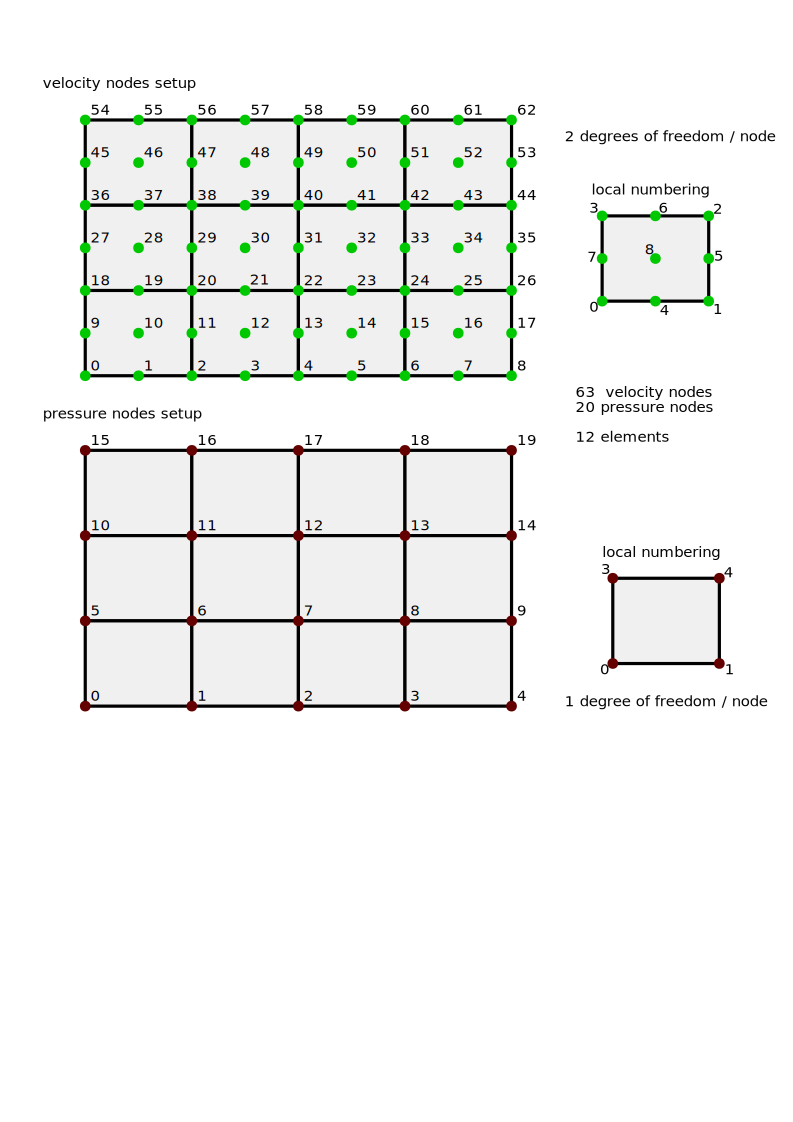
\includegraphics[width=10cm]{python_codes/fieldstone_18/images/q2q1setup}
\end{center}

%-----------------------------------------
\subsection*{Donea \& Huerta benchmark ({\tt bench=1})}
The details of the numerical setup are presented in Section \ref{MMM-mms1}.

\begin{center}
\includegraphics[width=7cm]{python_codes/fieldstone_18/results/mms/vel}
\includegraphics[width=7cm]{python_codes/fieldstone_18/results/mms/pressure}\\
{\captionfont Velocity and pressure fields for $32\times 32$ elements grid}
\end{center}

\begin{center}
\includegraphics[width=12cm]{python_codes/fieldstone_18/results/mms/errors}\\
{\captionfont Velocity and pressure error convergence for both nullspace removal 
techniques. The zero average pressure approach yields smaller errors.}
\end{center}

\newpage
%-----------------------------------------
\subsection*{Burman \& Hansbo manufactured solution ({\tt bench=4})}

The details of the numerical setup are presented in Section \ref{MMM-ss:mms_buha06}.
The velocity and pressure fields are given in the unit square by
\begin{eqnarray}
u(x,y) &=& 20xy^3 \nn\\
v(x,y) &=& 5x^4-5y^4 \nn\\
p(x,y) &=& 60x^2y -20y^3 -5
\end{eqnarray}
The analytical velocity is prescribed on all sides of the domain.

\begin{center}
\includegraphics[width=7cm]{python_codes/fieldstone_18/results/buha06/vel}
\includegraphics[width=7cm]{python_codes/fieldstone_18/results/buha06/p}\\
{\captionfont Velocity and pressure fields for $64\times 64$ elements grid}
\end{center}

\begin{center}
\includegraphics[width=8cm]{python_codes/fieldstone_18/results/buha06/errorsV}
\includegraphics[width=8cm]{python_codes/fieldstone_18/results/buha06/errorsP}\\
{\captionfont Velocity and pressure error convergence. Zero average.}
\end{center}

The conclusion is clear (and expected): there is no good reason 
to run such higher numbers of quadrature points.


\newpage
%----------------------------------------------------
\subsection*{Stokes sphere benchmark ({\tt bench=2})}

The setup is described in Section~\ref{MMM-ss:stokes_sphere2D}.
The domain is the unit square.
A sphere of radius 0.123456789 is placed in the middle of the domain. 
Its density is 1.01 while the density of the surrounding fluid is 1,
while its viscosity is 1000 times larger than the viscosity of the fluid.
Gravity is pointing downward with $|g|=1$.
There is no analytical solution to this problem.
Either no-slip or free-slip boundary conditions are prescribed on all 
sides.

\subsubsection*{Free-slip boundary conditions (FS)}

\begin{center}
\includegraphics[width=5.7cm]{python_codes/fieldstone_18/results/sphere/FS/vel}
\includegraphics[width=5.7cm]{python_codes/fieldstone_18/results/sphere/FS/press}
\includegraphics[width=5.7cm]{python_codes/fieldstone_18/results/sphere/FS/divv}\\
{\captionfont Velocity, pressure and velocity divergence fields for $48\times 48$ 
elements grid and $3^2$ quadrature points per element.}
\end{center}






\subsubsection*{No-slip boundary conditions (NS)}

\begin{center}
\includegraphics[width=5.7cm]{python_codes/fieldstone_18/results/sphere/NS/vel}
\includegraphics[width=5.7cm]{python_codes/fieldstone_18/results/sphere/NS/press}
\includegraphics[width=5.7cm]{python_codes/fieldstone_18/results/sphere/NS/divv}\\
{\captionfont Velocity, pressure and velocity divergence fields for $48\times 48$ 
elements grid and $3^2$ quadrature points per element.}
\end{center}




\newpage
%-----------------------------------------
\subsection*{Sinking block benchmark ({\tt bench=3})}

The setup is described in Section~\ref{MMM-ss:sinking_block} of part 1.
The domain is the unit square.
A block of density $\rho=1.01$ is placed in a fluid of density $\rho=1$.
The gravity is vertical and pointing downward with $|\vec{g}|=1$.
The function for $b_y$ is then:
\begin{lstlisting}
def by(x,y):
    [...]
    if abs(x-.5)<0.0625 and abs(y-0.5)<0.0625:
       val=-1.01
   else:
      val=-1.
\end{lstlisting}
The block is 1000 times more viscous than the fluid:
\begin{lstlisting}
def eta(x,y):
    [...]
    if bench==3:
       if abs(x-.5)<0.0625 and abs(y-0.5)<0.0625:
          val=1000
       else:
          val=1
\end{lstlisting}





\subsubsection*{Free slip boundary conditions (FS)}

\begin{center}
\includegraphics[width=7cm]{python_codes/fieldstone_18/results/block/FS/vel}
\includegraphics[width=7cm]{python_codes/fieldstone_18/results/block/FS/press}\\
{\captionfont Velocity and pressure fields for $48\times 48$ elements grid and $3^2$
quadrature points per element.}
\end{center}


\begin{center}
\includegraphics[width=5.7cm]{python_codes/fieldstone_18/results/block/vrms}
\includegraphics[width=5.7cm]{python_codes/fieldstone_18/results/block/max_vel}\\
\includegraphics[width=5.7cm]{python_codes/fieldstone_18/results/block/min_u}
\includegraphics[width=5.7cm]{python_codes/fieldstone_18/results/block/max_u}\\
\includegraphics[width=5.7cm]{python_codes/fieldstone_18/results/block/min_v}
\includegraphics[width=5.7cm]{python_codes/fieldstone_18/results/block/max_v}\\
\includegraphics[width=5.7cm]{python_codes/fieldstone_18/results/block/min_p}
\includegraphics[width=5.7cm]{python_codes/fieldstone_18/results/block/max_p}\\
\includegraphics[width=5.7cm]{python_codes/fieldstone_18/results/block/profile_u_FS}
\includegraphics[width=5.7cm]{python_codes/fieldstone_18/results/block/profile_v_FS}
\includegraphics[width=5.7cm]{python_codes/fieldstone_18/results/block/profile_p_FS}
\end{center}

%.....................................................
\subsubsection*{No slip boundary conditions (NS)}

\begin{center}
\includegraphics[width=5.7cm]{python_codes/fieldstone_18/results/block/NS/u}
\includegraphics[width=5.7cm]{python_codes/fieldstone_18/results/block/NS/v}
\includegraphics[width=5.7cm]{python_codes/fieldstone_18/results/block/NS/p}\\
{\captionfont Velocity and pressure fields for $32\times 32$ elements grid and $3^2$
quadrature points per element.}
\end{center}

Velocity and pressure are also measured on a vertical line going through
the middle of the domain/block (the lithostatic pressure is 
subtracted from the computed full pressure so that what is plotted is the 
dynamic pressure):
\begin{center}
\includegraphics[width=5.7cm]{python_codes/fieldstone_18/results/block/profile_u_NS}
\includegraphics[width=5.7cm]{python_codes/fieldstone_18/results/block/profile_v_NS}
\includegraphics[width=5.7cm]{python_codes/fieldstone_18/results/block/profile_p_NS}
\end{center}
As expected, the $x$ component of the velocity is zero because of symmetry.


\newpage
%----------------------------------------------------
\subsection*{Inclusion in pure shear ({\tt bench=5})}

(this setup was created for Philippe Yamato of Rennes University)

The inclusion is placed at the origin and has a radius 0.1, while the domain is the 
unit square. Viscosity inside the inclusion is 1 while the matrix viscosity is 1000.
Free slip is prescribed on the left and bottom boundary while 
$u=-1$ is prescribed on the right boundary and $v=+1$ on the top.

\begin{center}
\includegraphics[width=5.7cm]{python_codes/fieldstone_18/results/inclusion/eta}
\includegraphics[width=5.7cm]{python_codes/fieldstone_18/results/inclusion/vel}
\includegraphics[width=5.7cm]{python_codes/fieldstone_18/results/inclusion/press}\\
{\captionfont Resolution $256\times 256$.}
\end{center}

Note that viscosity is prescribed on quadrature levels, which in this case 
is likely to generate large errors/jumps around the inclusion surface.

\begin{verbatim}
For 256x256 mesh on my laptop:
setup: grid points: 0.128 s
setup: connectivity: 0.242 s
setup: boundary conditions: 0.151 s
build FE matrix: 284.284 s
assemble blocks: 0.003 s
solve time: 804.607 s
\end{verbatim}





\newpage
%%%%%%%%%%%%%%%%%%%%%%%%%%%%%%%%%%%%%%%%%%%%%%%%%%%%%%%%%%%%%%%%%%%%%%%%%%%%%%%
\section{{\tt fieldstone}: solvi benchmark}
\includegraphics[height=1.25cm]{images/pictograms/benchmark}
\includegraphics[height=1.25cm]{images/pictograms/FEM}

%%%%%%%%%%%%%%%%%%%%%%%%%%%%%%%%%%%%%%%%%%%%%%%%%%%%%%%%%%%%%%%%%%%%%%%%%%%%%%%%%%%%%%%%%%%%%%%%%%%

%\lstinputlisting[language=bash,basicstyle=\small]{python_codes/fieldstone_18/keywords.key}

\begin{center}
\inpython
{\small Code: \url{https://github.com/cedrict/fieldstone/tree/master/python_codes/fieldstone_18}}
\end{center}

\par\noindent\rule{\textwidth}{0.4pt}

Last revision: Feb. 7th, 2025.

\par\noindent\rule{\textwidth}{0.4pt}

%%%%%%%%%%%%%%%%%%%%%%%%%%%%%%%%%%%%%%%%%%%%%%%%%%%%%%%%%%%%%%%%%%%%%%%%%%%%%%%%%%%%%%%%%%%%%%%%%%%

The code relies on \QtwoQone elements.
Each element has $m_V=9$ vertices so in total $ndof_V\times m_V=18$ velocity dofs and 
$ndof_P*m_P=4$ pressure dofs. The total number of 
velocity dofs is therefore $NfemV=NV \times ndofV$ while the total number of
pressure dofs is $NfemP=NP\times ndofP$. The total number of dofs is then $Nfem=NfemV+NfemP$.

As a consequence, matrix $\K$ has size $NfemV,NfemV$ and matrix $\G$ has size $NfemV,NfemP$.
Vector $f$ is of size $NfemV$ and vector $h$ is of size $NfemP$.  

When needed the pressure nullspace is removed 
by imposing (Lagrange multiplier) that $\int_\Omega p \; dV=0$.

The following figure shows the layout of velocity and pressure nodes
for a $4\times 3$ element mesh:
\begin{center}
\includegraphics[width=10cm]{python_codes/fieldstone_18/images/q2q1setup}
\end{center}

%-----------------------------------------
\subsection*{Donea \& Huerta benchmark ({\tt bench=1})}
The details of the numerical setup are presented in Section \ref{MMM-mms1}.

\begin{center}
\includegraphics[width=7cm]{python_codes/fieldstone_18/results/mms/vel}
\includegraphics[width=7cm]{python_codes/fieldstone_18/results/mms/pressure}\\
{\captionfont Velocity and pressure fields for $32\times 32$ elements grid}
\end{center}

\begin{center}
\includegraphics[width=12cm]{python_codes/fieldstone_18/results/mms/errors}\\
{\captionfont Velocity and pressure error convergence for both nullspace removal 
techniques. The zero average pressure approach yields smaller errors.}
\end{center}

\newpage
%-----------------------------------------
\subsection*{Burman \& Hansbo manufactured solution ({\tt bench=4})}

The details of the numerical setup are presented in Section \ref{MMM-ss:mms_buha06}.
The velocity and pressure fields are given in the unit square by
\begin{eqnarray}
u(x,y) &=& 20xy^3 \nn\\
v(x,y) &=& 5x^4-5y^4 \nn\\
p(x,y) &=& 60x^2y -20y^3 -5
\end{eqnarray}
The analytical velocity is prescribed on all sides of the domain.

\begin{center}
\includegraphics[width=7cm]{python_codes/fieldstone_18/results/buha06/vel}
\includegraphics[width=7cm]{python_codes/fieldstone_18/results/buha06/p}\\
{\captionfont Velocity and pressure fields for $64\times 64$ elements grid}
\end{center}

\begin{center}
\includegraphics[width=8cm]{python_codes/fieldstone_18/results/buha06/errorsV}
\includegraphics[width=8cm]{python_codes/fieldstone_18/results/buha06/errorsP}\\
{\captionfont Velocity and pressure error convergence. Zero average.}
\end{center}

The conclusion is clear (and expected): there is no good reason 
to run such higher numbers of quadrature points.


\newpage
%----------------------------------------------------
\subsection*{Stokes sphere benchmark ({\tt bench=2})}

The setup is described in Section~\ref{MMM-ss:stokes_sphere2D}.
The domain is the unit square.
A sphere of radius 0.123456789 is placed in the middle of the domain. 
Its density is 1.01 while the density of the surrounding fluid is 1,
while its viscosity is 1000 times larger than the viscosity of the fluid.
Gravity is pointing downward with $|g|=1$.
There is no analytical solution to this problem.
Either no-slip or free-slip boundary conditions are prescribed on all 
sides.

\subsubsection*{Free-slip boundary conditions (FS)}

\begin{center}
\includegraphics[width=5.7cm]{python_codes/fieldstone_18/results/sphere/FS/vel}
\includegraphics[width=5.7cm]{python_codes/fieldstone_18/results/sphere/FS/press}
\includegraphics[width=5.7cm]{python_codes/fieldstone_18/results/sphere/FS/divv}\\
{\captionfont Velocity, pressure and velocity divergence fields for $48\times 48$ 
elements grid and $3^2$ quadrature points per element.}
\end{center}






\subsubsection*{No-slip boundary conditions (NS)}

\begin{center}
\includegraphics[width=5.7cm]{python_codes/fieldstone_18/results/sphere/NS/vel}
\includegraphics[width=5.7cm]{python_codes/fieldstone_18/results/sphere/NS/press}
\includegraphics[width=5.7cm]{python_codes/fieldstone_18/results/sphere/NS/divv}\\
{\captionfont Velocity, pressure and velocity divergence fields for $48\times 48$ 
elements grid and $3^2$ quadrature points per element.}
\end{center}




\newpage
%-----------------------------------------
\subsection*{Sinking block benchmark ({\tt bench=3})}

The setup is described in Section~\ref{MMM-ss:sinking_block} of part 1.
The domain is the unit square.
A block of density $\rho=1.01$ is placed in a fluid of density $\rho=1$.
The gravity is vertical and pointing downward with $|\vec{g}|=1$.
The function for $b_y$ is then:
\begin{lstlisting}
def by(x,y):
    [...]
    if abs(x-.5)<0.0625 and abs(y-0.5)<0.0625:
       val=-1.01
   else:
      val=-1.
\end{lstlisting}
The block is 1000 times more viscous than the fluid:
\begin{lstlisting}
def eta(x,y):
    [...]
    if bench==3:
       if abs(x-.5)<0.0625 and abs(y-0.5)<0.0625:
          val=1000
       else:
          val=1
\end{lstlisting}





\subsubsection*{Free slip boundary conditions (FS)}

\begin{center}
\includegraphics[width=7cm]{python_codes/fieldstone_18/results/block/FS/vel}
\includegraphics[width=7cm]{python_codes/fieldstone_18/results/block/FS/press}\\
{\captionfont Velocity and pressure fields for $48\times 48$ elements grid and $3^2$
quadrature points per element.}
\end{center}


\begin{center}
\includegraphics[width=5.7cm]{python_codes/fieldstone_18/results/block/vrms}
\includegraphics[width=5.7cm]{python_codes/fieldstone_18/results/block/max_vel}\\
\includegraphics[width=5.7cm]{python_codes/fieldstone_18/results/block/min_u}
\includegraphics[width=5.7cm]{python_codes/fieldstone_18/results/block/max_u}\\
\includegraphics[width=5.7cm]{python_codes/fieldstone_18/results/block/min_v}
\includegraphics[width=5.7cm]{python_codes/fieldstone_18/results/block/max_v}\\
\includegraphics[width=5.7cm]{python_codes/fieldstone_18/results/block/min_p}
\includegraphics[width=5.7cm]{python_codes/fieldstone_18/results/block/max_p}\\
\includegraphics[width=5.7cm]{python_codes/fieldstone_18/results/block/profile_u_FS}
\includegraphics[width=5.7cm]{python_codes/fieldstone_18/results/block/profile_v_FS}
\includegraphics[width=5.7cm]{python_codes/fieldstone_18/results/block/profile_p_FS}
\end{center}

%.....................................................
\subsubsection*{No slip boundary conditions (NS)}

\begin{center}
\includegraphics[width=5.7cm]{python_codes/fieldstone_18/results/block/NS/u}
\includegraphics[width=5.7cm]{python_codes/fieldstone_18/results/block/NS/v}
\includegraphics[width=5.7cm]{python_codes/fieldstone_18/results/block/NS/p}\\
{\captionfont Velocity and pressure fields for $32\times 32$ elements grid and $3^2$
quadrature points per element.}
\end{center}

Velocity and pressure are also measured on a vertical line going through
the middle of the domain/block (the lithostatic pressure is 
subtracted from the computed full pressure so that what is plotted is the 
dynamic pressure):
\begin{center}
\includegraphics[width=5.7cm]{python_codes/fieldstone_18/results/block/profile_u_NS}
\includegraphics[width=5.7cm]{python_codes/fieldstone_18/results/block/profile_v_NS}
\includegraphics[width=5.7cm]{python_codes/fieldstone_18/results/block/profile_p_NS}
\end{center}
As expected, the $x$ component of the velocity is zero because of symmetry.


\newpage
%----------------------------------------------------
\subsection*{Inclusion in pure shear ({\tt bench=5})}

(this setup was created for Philippe Yamato of Rennes University)

The inclusion is placed at the origin and has a radius 0.1, while the domain is the 
unit square. Viscosity inside the inclusion is 1 while the matrix viscosity is 1000.
Free slip is prescribed on the left and bottom boundary while 
$u=-1$ is prescribed on the right boundary and $v=+1$ on the top.

\begin{center}
\includegraphics[width=5.7cm]{python_codes/fieldstone_18/results/inclusion/eta}
\includegraphics[width=5.7cm]{python_codes/fieldstone_18/results/inclusion/vel}
\includegraphics[width=5.7cm]{python_codes/fieldstone_18/results/inclusion/press}\\
{\captionfont Resolution $256\times 256$.}
\end{center}

Note that viscosity is prescribed on quadrature levels, which in this case 
is likely to generate large errors/jumps around the inclusion surface.

\begin{verbatim}
For 256x256 mesh on my laptop:
setup: grid points: 0.128 s
setup: connectivity: 0.242 s
setup: boundary conditions: 0.151 s
build FE matrix: 284.284 s
assemble blocks: 0.003 s
solve time: 804.607 s
\end{verbatim}





\newpage
%%%%%%%%%%%%%%%%%%%%%%%%%%%%%%%%%%%%%%%%%%%%%%%%%%%%%%%%%%%%%%%%%%%%%%%%%%%%%%%
\section{{\tt fieldstone}: the indentor benchmark}

The punch benchmark is one of the few boundary value problems involving plastic solids for which there exists an exact solution. 
Such solutions are usually either for highly simplified geometries (spherical or axial symmetry, for instance) or simplified material models (such as rigid plastic solids) \cite{kacha04}.

In this experiment, a rigid punch indents a rigid plastic half space; the slip line field theory gives 
exact solutions as shown in Fig. \ref{fig_punch}a. 
The plane strain formulation of the equations and the detailed solution to the problem were derived in the Appendix of \cite{thfb08} and are also presented in \cite{gepd98}.

The two dimensional punch problem has been extensively studied numerically for the past 40 years 
\cite{zihl75,zihp95,chpe01,chan99,huhy99,yuti06,bufs08,raab07} and has been used to draw a parallel with the tectonics of eastern China in the context of the 
India-Eurasia collision \cite{tamo76,mota77}.
It is also worth noting that it has been carried out in one form or another in series of 
analogue modelling articles 
concerning the same region, with a rigid indenter colliding with a rheologically stratified lithosphere \cite{peta88,daco88,jodc90}.

 
Numerically, the one-time step punch experiment is performed on a two-dimensional
domain of purely plastic von Mises material. 
Given that the von Mises rheology yield criterion does not depend on pressure, the density of the material and/or the gravity vector is set to zero. Sides are set to free slip boundary conditions, the bottom to no slip, while a vertical velocity $(0,-v_p)$ is prescribed at the top boundary for nodes whose $x$ coordinate is within $[L_x/2-\delta/2,L_x/2+\delta/2]$. 

The following parameters are used: $L_x=1$, $L_y=0.5$, $\mu_{min}=10^{-3}$, 
$\mu_{max}=10^3$, $v_p=1$, $\delta=0.123456789$ 
and the yield value of the material is set to $k=1$. 

The analytical solution predicts that the angle of the shear bands stemming from the sides of the punch 
is $\pi/4$, that the pressure right under the punch is $1+\pi$, 
and that the velocity of the rigid blocks on each side of the punch is $v_p/\sqrt{2}$ 
(this is simply explained by invoking conservation of mass).

\includegraphics[width=16cm]{python_codes/fieldstone_indentor/solution.pdf}

ToDo: smooth punch

\fbox{
\parbox{10cm}{{\bf features}
\begin{itemize}
\item $Q_1\times P_0$ element \index{$Q_1 \times P_0$}
\item incompressible flow \index{incompressible flow}
\item penalty formulation \index{penalty formulation}
\item Dirichlet boundary conditions (no-slip)
\item isothermal \index{isothermal}
\item non-isoviscous \index{non-isoviscous}
\item nonlinear rheology \index{nonlinear rheology}
\end{itemize}
}}



\newpage
%%%%%%%%%%%%%%%%%%%%%%%%%%%%%%%%%%%%%%%%%%%%%%%%%%%%%%%%%%%%%%%%%%%%%%%%%%%%%%%
\section{{\tt fieldstone}: the annulus benchmark}
\includegraphics[height=1.25cm]{images/pictograms/benchmark}
\includegraphics[height=1.25cm]{images/pictograms/FEM}

%%%%%%%%%%%%%%%%%%%%%%%%%%%%%%%%%%%%%%%%%%%%%%%%%%%%%%%%%%%%%%%%%%%%%%%%%%%%%%%%%%%%%%%%%%%%%%%%%%%

%\lstinputlisting[language=bash,basicstyle=\small]{python_codes/fieldstone_18/keywords.key}

\begin{center}
\inpython
{\small Code: \url{https://github.com/cedrict/fieldstone/tree/master/python_codes/fieldstone_18}}
\end{center}

\par\noindent\rule{\textwidth}{0.4pt}

Last revision: Feb. 7th, 2025.

\par\noindent\rule{\textwidth}{0.4pt}

%%%%%%%%%%%%%%%%%%%%%%%%%%%%%%%%%%%%%%%%%%%%%%%%%%%%%%%%%%%%%%%%%%%%%%%%%%%%%%%%%%%%%%%%%%%%%%%%%%%

The code relies on \QtwoQone elements.
Each element has $m_V=9$ vertices so in total $ndof_V\times m_V=18$ velocity dofs and 
$ndof_P*m_P=4$ pressure dofs. The total number of 
velocity dofs is therefore $NfemV=NV \times ndofV$ while the total number of
pressure dofs is $NfemP=NP\times ndofP$. The total number of dofs is then $Nfem=NfemV+NfemP$.

As a consequence, matrix $\K$ has size $NfemV,NfemV$ and matrix $\G$ has size $NfemV,NfemP$.
Vector $f$ is of size $NfemV$ and vector $h$ is of size $NfemP$.  

When needed the pressure nullspace is removed 
by imposing (Lagrange multiplier) that $\int_\Omega p \; dV=0$.

The following figure shows the layout of velocity and pressure nodes
for a $4\times 3$ element mesh:
\begin{center}
\includegraphics[width=10cm]{python_codes/fieldstone_18/images/q2q1setup}
\end{center}

%-----------------------------------------
\subsection*{Donea \& Huerta benchmark ({\tt bench=1})}
The details of the numerical setup are presented in Section \ref{MMM-mms1}.

\begin{center}
\includegraphics[width=7cm]{python_codes/fieldstone_18/results/mms/vel}
\includegraphics[width=7cm]{python_codes/fieldstone_18/results/mms/pressure}\\
{\captionfont Velocity and pressure fields for $32\times 32$ elements grid}
\end{center}

\begin{center}
\includegraphics[width=12cm]{python_codes/fieldstone_18/results/mms/errors}\\
{\captionfont Velocity and pressure error convergence for both nullspace removal 
techniques. The zero average pressure approach yields smaller errors.}
\end{center}

\newpage
%-----------------------------------------
\subsection*{Burman \& Hansbo manufactured solution ({\tt bench=4})}

The details of the numerical setup are presented in Section \ref{MMM-ss:mms_buha06}.
The velocity and pressure fields are given in the unit square by
\begin{eqnarray}
u(x,y) &=& 20xy^3 \nn\\
v(x,y) &=& 5x^4-5y^4 \nn\\
p(x,y) &=& 60x^2y -20y^3 -5
\end{eqnarray}
The analytical velocity is prescribed on all sides of the domain.

\begin{center}
\includegraphics[width=7cm]{python_codes/fieldstone_18/results/buha06/vel}
\includegraphics[width=7cm]{python_codes/fieldstone_18/results/buha06/p}\\
{\captionfont Velocity and pressure fields for $64\times 64$ elements grid}
\end{center}

\begin{center}
\includegraphics[width=8cm]{python_codes/fieldstone_18/results/buha06/errorsV}
\includegraphics[width=8cm]{python_codes/fieldstone_18/results/buha06/errorsP}\\
{\captionfont Velocity and pressure error convergence. Zero average.}
\end{center}

The conclusion is clear (and expected): there is no good reason 
to run such higher numbers of quadrature points.


\newpage
%----------------------------------------------------
\subsection*{Stokes sphere benchmark ({\tt bench=2})}

The setup is described in Section~\ref{MMM-ss:stokes_sphere2D}.
The domain is the unit square.
A sphere of radius 0.123456789 is placed in the middle of the domain. 
Its density is 1.01 while the density of the surrounding fluid is 1,
while its viscosity is 1000 times larger than the viscosity of the fluid.
Gravity is pointing downward with $|g|=1$.
There is no analytical solution to this problem.
Either no-slip or free-slip boundary conditions are prescribed on all 
sides.

\subsubsection*{Free-slip boundary conditions (FS)}

\begin{center}
\includegraphics[width=5.7cm]{python_codes/fieldstone_18/results/sphere/FS/vel}
\includegraphics[width=5.7cm]{python_codes/fieldstone_18/results/sphere/FS/press}
\includegraphics[width=5.7cm]{python_codes/fieldstone_18/results/sphere/FS/divv}\\
{\captionfont Velocity, pressure and velocity divergence fields for $48\times 48$ 
elements grid and $3^2$ quadrature points per element.}
\end{center}






\subsubsection*{No-slip boundary conditions (NS)}

\begin{center}
\includegraphics[width=5.7cm]{python_codes/fieldstone_18/results/sphere/NS/vel}
\includegraphics[width=5.7cm]{python_codes/fieldstone_18/results/sphere/NS/press}
\includegraphics[width=5.7cm]{python_codes/fieldstone_18/results/sphere/NS/divv}\\
{\captionfont Velocity, pressure and velocity divergence fields for $48\times 48$ 
elements grid and $3^2$ quadrature points per element.}
\end{center}




\newpage
%-----------------------------------------
\subsection*{Sinking block benchmark ({\tt bench=3})}

The setup is described in Section~\ref{MMM-ss:sinking_block} of part 1.
The domain is the unit square.
A block of density $\rho=1.01$ is placed in a fluid of density $\rho=1$.
The gravity is vertical and pointing downward with $|\vec{g}|=1$.
The function for $b_y$ is then:
\begin{lstlisting}
def by(x,y):
    [...]
    if abs(x-.5)<0.0625 and abs(y-0.5)<0.0625:
       val=-1.01
   else:
      val=-1.
\end{lstlisting}
The block is 1000 times more viscous than the fluid:
\begin{lstlisting}
def eta(x,y):
    [...]
    if bench==3:
       if abs(x-.5)<0.0625 and abs(y-0.5)<0.0625:
          val=1000
       else:
          val=1
\end{lstlisting}





\subsubsection*{Free slip boundary conditions (FS)}

\begin{center}
\includegraphics[width=7cm]{python_codes/fieldstone_18/results/block/FS/vel}
\includegraphics[width=7cm]{python_codes/fieldstone_18/results/block/FS/press}\\
{\captionfont Velocity and pressure fields for $48\times 48$ elements grid and $3^2$
quadrature points per element.}
\end{center}


\begin{center}
\includegraphics[width=5.7cm]{python_codes/fieldstone_18/results/block/vrms}
\includegraphics[width=5.7cm]{python_codes/fieldstone_18/results/block/max_vel}\\
\includegraphics[width=5.7cm]{python_codes/fieldstone_18/results/block/min_u}
\includegraphics[width=5.7cm]{python_codes/fieldstone_18/results/block/max_u}\\
\includegraphics[width=5.7cm]{python_codes/fieldstone_18/results/block/min_v}
\includegraphics[width=5.7cm]{python_codes/fieldstone_18/results/block/max_v}\\
\includegraphics[width=5.7cm]{python_codes/fieldstone_18/results/block/min_p}
\includegraphics[width=5.7cm]{python_codes/fieldstone_18/results/block/max_p}\\
\includegraphics[width=5.7cm]{python_codes/fieldstone_18/results/block/profile_u_FS}
\includegraphics[width=5.7cm]{python_codes/fieldstone_18/results/block/profile_v_FS}
\includegraphics[width=5.7cm]{python_codes/fieldstone_18/results/block/profile_p_FS}
\end{center}

%.....................................................
\subsubsection*{No slip boundary conditions (NS)}

\begin{center}
\includegraphics[width=5.7cm]{python_codes/fieldstone_18/results/block/NS/u}
\includegraphics[width=5.7cm]{python_codes/fieldstone_18/results/block/NS/v}
\includegraphics[width=5.7cm]{python_codes/fieldstone_18/results/block/NS/p}\\
{\captionfont Velocity and pressure fields for $32\times 32$ elements grid and $3^2$
quadrature points per element.}
\end{center}

Velocity and pressure are also measured on a vertical line going through
the middle of the domain/block (the lithostatic pressure is 
subtracted from the computed full pressure so that what is plotted is the 
dynamic pressure):
\begin{center}
\includegraphics[width=5.7cm]{python_codes/fieldstone_18/results/block/profile_u_NS}
\includegraphics[width=5.7cm]{python_codes/fieldstone_18/results/block/profile_v_NS}
\includegraphics[width=5.7cm]{python_codes/fieldstone_18/results/block/profile_p_NS}
\end{center}
As expected, the $x$ component of the velocity is zero because of symmetry.


\newpage
%----------------------------------------------------
\subsection*{Inclusion in pure shear ({\tt bench=5})}

(this setup was created for Philippe Yamato of Rennes University)

The inclusion is placed at the origin and has a radius 0.1, while the domain is the 
unit square. Viscosity inside the inclusion is 1 while the matrix viscosity is 1000.
Free slip is prescribed on the left and bottom boundary while 
$u=-1$ is prescribed on the right boundary and $v=+1$ on the top.

\begin{center}
\includegraphics[width=5.7cm]{python_codes/fieldstone_18/results/inclusion/eta}
\includegraphics[width=5.7cm]{python_codes/fieldstone_18/results/inclusion/vel}
\includegraphics[width=5.7cm]{python_codes/fieldstone_18/results/inclusion/press}\\
{\captionfont Resolution $256\times 256$.}
\end{center}

Note that viscosity is prescribed on quadrature levels, which in this case 
is likely to generate large errors/jumps around the inclusion surface.

\begin{verbatim}
For 256x256 mesh on my laptop:
setup: grid points: 0.128 s
setup: connectivity: 0.242 s
setup: boundary conditions: 0.151 s
build FE matrix: 284.284 s
assemble blocks: 0.003 s
solve time: 804.607 s
\end{verbatim}






\newpage
%%%%%%%%%%%%%%%%%%%%%%%%%%%%%%%%%%%%%%%%%%%%%%%%%%%%%%%%%%%%%%%%%%%%%%%%%%%%%%%
\section{{\tt fieldstone}: stokes sphere (3D)}

\fbox{
\parbox{10cm}{{\bf features}
\begin{itemize}
\item $Q_1\times P_0$ element
\item incompressible flow
\item penalty formulation
\item Dirichlet boundary conditions (free-slip)
\item direct solver
\item isothermal
\item non-isoviscous
\item 3D
\item elemental b.c. 
\item buoyancy driven
\end{itemize}
}}


\begin{center}
\includegraphics[width=5cm]{python_codes/fieldstone_stokes_sphere_3D/grid}
\includegraphics[width=5cm]{python_codes/fieldstone_stokes_sphere_3D/vel}
\includegraphics[width=5cm]{python_codes/fieldstone_stokes_sphere_3D/press}\\
\includegraphics[width=5cm]{python_codes/fieldstone_stokes_sphere_3D/press2}
\includegraphics[width=5cm]{python_codes/fieldstone_stokes_sphere_3D/visc}
\includegraphics[width=5cm]{python_codes/fieldstone_stokes_sphere_3D/dens}\\
{\small resolution is 24x24x24}
\end{center}



\newpage
%%%%%%%%%%%%%%%%%%%%%%%%%%%%%%%%%%%%%%%%%%%%%%%%%%%%%%%%%%%%%%%%%%%%%%%%%%%%%%%
\section{{\tt fieldstone}: consistent pressure recovery }


\[
p = -\lambda {\bm \nabla}\cdot {\bm v}
\]

$q_1$ is smoothed pressure obtained with the  center-to-node approach.

$q_2$ is recovered pressure obtained with \cite{zina82}.

All three fulfill the zero average condition: $\int p d\Omega = 0$.

\includegraphics[width=15cm]{python_codes/fieldstone_consistent_pressure_recovery/solution}

\includegraphics[width=8cm]{python_codes/fieldstone_consistent_pressure_recovery/errors}

In terms of pressure error, $q_2$ is better than $q_1$ which is better than elemental.

QUESTION: why are the averages exactly zero ?!

TODO: 
\begin{itemize}
\item add randomness to internal node positions.
\item look at elefant algorithms
\end{itemize}


\newpage
%%%%%%%%%%%%%%%%%%%%%%%%%%%%%%%%%%%%%%%%%%%%%%%%%%%%%%%%%%%%%%%%%%%%%%%%%%%%%%%
\section{{\tt fieldstone}: the Particle in Cell technique (1) - the effect of averaging}
\includegraphics[height=1.25cm]{images/pictograms/benchmark}
\includegraphics[height=1.25cm]{images/pictograms/FEM}

%%%%%%%%%%%%%%%%%%%%%%%%%%%%%%%%%%%%%%%%%%%%%%%%%%%%%%%%%%%%%%%%%%%%%%%%%%%%%%%%%%%%%%%%%%%%%%%%%%%

%\lstinputlisting[language=bash,basicstyle=\small]{python_codes/fieldstone_18/keywords.key}

\begin{center}
\inpython
{\small Code: \url{https://github.com/cedrict/fieldstone/tree/master/python_codes/fieldstone_18}}
\end{center}

\par\noindent\rule{\textwidth}{0.4pt}

Last revision: Feb. 7th, 2025.

\par\noindent\rule{\textwidth}{0.4pt}

%%%%%%%%%%%%%%%%%%%%%%%%%%%%%%%%%%%%%%%%%%%%%%%%%%%%%%%%%%%%%%%%%%%%%%%%%%%%%%%%%%%%%%%%%%%%%%%%%%%

The code relies on \QtwoQone elements.
Each element has $m_V=9$ vertices so in total $ndof_V\times m_V=18$ velocity dofs and 
$ndof_P*m_P=4$ pressure dofs. The total number of 
velocity dofs is therefore $NfemV=NV \times ndofV$ while the total number of
pressure dofs is $NfemP=NP\times ndofP$. The total number of dofs is then $Nfem=NfemV+NfemP$.

As a consequence, matrix $\K$ has size $NfemV,NfemV$ and matrix $\G$ has size $NfemV,NfemP$.
Vector $f$ is of size $NfemV$ and vector $h$ is of size $NfemP$.  

When needed the pressure nullspace is removed 
by imposing (Lagrange multiplier) that $\int_\Omega p \; dV=0$.

The following figure shows the layout of velocity and pressure nodes
for a $4\times 3$ element mesh:
\begin{center}
\includegraphics[width=10cm]{python_codes/fieldstone_18/images/q2q1setup}
\end{center}

%-----------------------------------------
\subsection*{Donea \& Huerta benchmark ({\tt bench=1})}
The details of the numerical setup are presented in Section \ref{MMM-mms1}.

\begin{center}
\includegraphics[width=7cm]{python_codes/fieldstone_18/results/mms/vel}
\includegraphics[width=7cm]{python_codes/fieldstone_18/results/mms/pressure}\\
{\captionfont Velocity and pressure fields for $32\times 32$ elements grid}
\end{center}

\begin{center}
\includegraphics[width=12cm]{python_codes/fieldstone_18/results/mms/errors}\\
{\captionfont Velocity and pressure error convergence for both nullspace removal 
techniques. The zero average pressure approach yields smaller errors.}
\end{center}

\newpage
%-----------------------------------------
\subsection*{Burman \& Hansbo manufactured solution ({\tt bench=4})}

The details of the numerical setup are presented in Section \ref{MMM-ss:mms_buha06}.
The velocity and pressure fields are given in the unit square by
\begin{eqnarray}
u(x,y) &=& 20xy^3 \nn\\
v(x,y) &=& 5x^4-5y^4 \nn\\
p(x,y) &=& 60x^2y -20y^3 -5
\end{eqnarray}
The analytical velocity is prescribed on all sides of the domain.

\begin{center}
\includegraphics[width=7cm]{python_codes/fieldstone_18/results/buha06/vel}
\includegraphics[width=7cm]{python_codes/fieldstone_18/results/buha06/p}\\
{\captionfont Velocity and pressure fields for $64\times 64$ elements grid}
\end{center}

\begin{center}
\includegraphics[width=8cm]{python_codes/fieldstone_18/results/buha06/errorsV}
\includegraphics[width=8cm]{python_codes/fieldstone_18/results/buha06/errorsP}\\
{\captionfont Velocity and pressure error convergence. Zero average.}
\end{center}

The conclusion is clear (and expected): there is no good reason 
to run such higher numbers of quadrature points.


\newpage
%----------------------------------------------------
\subsection*{Stokes sphere benchmark ({\tt bench=2})}

The setup is described in Section~\ref{MMM-ss:stokes_sphere2D}.
The domain is the unit square.
A sphere of radius 0.123456789 is placed in the middle of the domain. 
Its density is 1.01 while the density of the surrounding fluid is 1,
while its viscosity is 1000 times larger than the viscosity of the fluid.
Gravity is pointing downward with $|g|=1$.
There is no analytical solution to this problem.
Either no-slip or free-slip boundary conditions are prescribed on all 
sides.

\subsubsection*{Free-slip boundary conditions (FS)}

\begin{center}
\includegraphics[width=5.7cm]{python_codes/fieldstone_18/results/sphere/FS/vel}
\includegraphics[width=5.7cm]{python_codes/fieldstone_18/results/sphere/FS/press}
\includegraphics[width=5.7cm]{python_codes/fieldstone_18/results/sphere/FS/divv}\\
{\captionfont Velocity, pressure and velocity divergence fields for $48\times 48$ 
elements grid and $3^2$ quadrature points per element.}
\end{center}






\subsubsection*{No-slip boundary conditions (NS)}

\begin{center}
\includegraphics[width=5.7cm]{python_codes/fieldstone_18/results/sphere/NS/vel}
\includegraphics[width=5.7cm]{python_codes/fieldstone_18/results/sphere/NS/press}
\includegraphics[width=5.7cm]{python_codes/fieldstone_18/results/sphere/NS/divv}\\
{\captionfont Velocity, pressure and velocity divergence fields for $48\times 48$ 
elements grid and $3^2$ quadrature points per element.}
\end{center}




\newpage
%-----------------------------------------
\subsection*{Sinking block benchmark ({\tt bench=3})}

The setup is described in Section~\ref{MMM-ss:sinking_block} of part 1.
The domain is the unit square.
A block of density $\rho=1.01$ is placed in a fluid of density $\rho=1$.
The gravity is vertical and pointing downward with $|\vec{g}|=1$.
The function for $b_y$ is then:
\begin{lstlisting}
def by(x,y):
    [...]
    if abs(x-.5)<0.0625 and abs(y-0.5)<0.0625:
       val=-1.01
   else:
      val=-1.
\end{lstlisting}
The block is 1000 times more viscous than the fluid:
\begin{lstlisting}
def eta(x,y):
    [...]
    if bench==3:
       if abs(x-.5)<0.0625 and abs(y-0.5)<0.0625:
          val=1000
       else:
          val=1
\end{lstlisting}





\subsubsection*{Free slip boundary conditions (FS)}

\begin{center}
\includegraphics[width=7cm]{python_codes/fieldstone_18/results/block/FS/vel}
\includegraphics[width=7cm]{python_codes/fieldstone_18/results/block/FS/press}\\
{\captionfont Velocity and pressure fields for $48\times 48$ elements grid and $3^2$
quadrature points per element.}
\end{center}


\begin{center}
\includegraphics[width=5.7cm]{python_codes/fieldstone_18/results/block/vrms}
\includegraphics[width=5.7cm]{python_codes/fieldstone_18/results/block/max_vel}\\
\includegraphics[width=5.7cm]{python_codes/fieldstone_18/results/block/min_u}
\includegraphics[width=5.7cm]{python_codes/fieldstone_18/results/block/max_u}\\
\includegraphics[width=5.7cm]{python_codes/fieldstone_18/results/block/min_v}
\includegraphics[width=5.7cm]{python_codes/fieldstone_18/results/block/max_v}\\
\includegraphics[width=5.7cm]{python_codes/fieldstone_18/results/block/min_p}
\includegraphics[width=5.7cm]{python_codes/fieldstone_18/results/block/max_p}\\
\includegraphics[width=5.7cm]{python_codes/fieldstone_18/results/block/profile_u_FS}
\includegraphics[width=5.7cm]{python_codes/fieldstone_18/results/block/profile_v_FS}
\includegraphics[width=5.7cm]{python_codes/fieldstone_18/results/block/profile_p_FS}
\end{center}

%.....................................................
\subsubsection*{No slip boundary conditions (NS)}

\begin{center}
\includegraphics[width=5.7cm]{python_codes/fieldstone_18/results/block/NS/u}
\includegraphics[width=5.7cm]{python_codes/fieldstone_18/results/block/NS/v}
\includegraphics[width=5.7cm]{python_codes/fieldstone_18/results/block/NS/p}\\
{\captionfont Velocity and pressure fields for $32\times 32$ elements grid and $3^2$
quadrature points per element.}
\end{center}

Velocity and pressure are also measured on a vertical line going through
the middle of the domain/block (the lithostatic pressure is 
subtracted from the computed full pressure so that what is plotted is the 
dynamic pressure):
\begin{center}
\includegraphics[width=5.7cm]{python_codes/fieldstone_18/results/block/profile_u_NS}
\includegraphics[width=5.7cm]{python_codes/fieldstone_18/results/block/profile_v_NS}
\includegraphics[width=5.7cm]{python_codes/fieldstone_18/results/block/profile_p_NS}
\end{center}
As expected, the $x$ component of the velocity is zero because of symmetry.


\newpage
%----------------------------------------------------
\subsection*{Inclusion in pure shear ({\tt bench=5})}

(this setup was created for Philippe Yamato of Rennes University)

The inclusion is placed at the origin and has a radius 0.1, while the domain is the 
unit square. Viscosity inside the inclusion is 1 while the matrix viscosity is 1000.
Free slip is prescribed on the left and bottom boundary while 
$u=-1$ is prescribed on the right boundary and $v=+1$ on the top.

\begin{center}
\includegraphics[width=5.7cm]{python_codes/fieldstone_18/results/inclusion/eta}
\includegraphics[width=5.7cm]{python_codes/fieldstone_18/results/inclusion/vel}
\includegraphics[width=5.7cm]{python_codes/fieldstone_18/results/inclusion/press}\\
{\captionfont Resolution $256\times 256$.}
\end{center}

Note that viscosity is prescribed on quadrature levels, which in this case 
is likely to generate large errors/jumps around the inclusion surface.

\begin{verbatim}
For 256x256 mesh on my laptop:
setup: grid points: 0.128 s
setup: connectivity: 0.242 s
setup: boundary conditions: 0.151 s
build FE matrix: 284.284 s
assemble blocks: 0.003 s
solve time: 804.607 s
\end{verbatim}











%\newpage
%\subsection{Using MUMPS}
%\subsection{With periodic boundary conditions}
%\subsection{Different Cmat}
%\subsection{Penalty Uzawa formulation}
%\subsection{Powell-Hestenes iterations a la MILAMIN}
%\subsection{With temperature and phase change}
%\subsection{Conformal refinement}
%\subsection{Newton vs Picard solver}
%\subsection{With markers}
%\subsection{Stress b.c.}
%\subsection{open boundary conditions}
%\subsection{melt generation}
%after Schmeling paper
%\subsection{Consistent pressure recovery}
%\subsection{Uzawa outer scheme}
%\subsection{PCG outer scheme}


\appendix

\newpage
%%%%%%%%%%%%%%%%%%%%%%%%%%%%%%%%%%%%%%%%%%%%%%%%%%%%%%%%%%%%%%%%%%%%%%%%%%%%%%%
\section{The main codes in computational geodynamics}

In what follows I make a quick inventory of the main codes of computational geodynamics, 
for crust, lithosphere and/or mantle modelling.

\subsection{ADELI}

\subsection{ASPECT}

\subsection{CITCOMS and CITCOMCU}

\subsection{DOUAR}

\subsection{GAIA}

\subsection{GALE}

\subsection{GTECTON}

\subsection{ELVIS}

\subsection{ELEFANT}

\subsection{ELLIPSIS}

\subsection{FANTOM}

\subsection{FLUIDITY}

\subsection{LAMEM}

\subsection{MILAMIN}

\subsection{PARAVOZ/FLAMAR}

\subsection{PTATIN}

\subsection{RHEA}

\subsection{SEPRAN}

\subsection{SOPALE}

\subsection{STAGYY}

\subsection{SULEC}
SULEC is a finite element code that solves the incompressible Navier-Stokes equations 
for slow creeping flows. The code is developed by Susan Ellis 
(GNS Sciences, NZ) and Susanne Buiter (NGU). 


\subsection{TERRA}

\subsection{UNDERWORLD 1\&2}




\newpage
%%%%%%%%%%%%%%%%%%%%%%%%%%%%%%%%%%%%%%%%%%%%%%%%%%%%%%%%%%%%%%%%%%%%%%%%%%%%%%%
\section{fieldstone.py}
%\lstinputlisting{python_codes/fieldstone/fieldstone.py}

\newpage
%%%%%%%%%%%%%%%%%%%%%%%%%%%%%%%%%%%%%%%%%%%%%%%%%%%%%%%%%%%%%%%%%%%%%%%%%%%%%%%
\section{fieldstone\_stokes\_sphere.py}
%\lstinputlisting{python_codes/fieldstone_stokes_sphere/fieldstone.py}

%%%%%%%%%%%%%%%%%%%%%%%%%%%%%%%%%%%%%%%%%%%%%%%%%%%%%%%%%%%%%%%%%%%%%%%%%%%%%%%
\section{fieldstone\_convection\_box.py}
%\lstinputlisting{python_codes/fieldstone_convection_box/fieldstone_convection_box.py}

\newpage
%%%%%%%%%%%%%%%%%%%%%%%%%%%%%%%%%%%%%%%%%%%%%%%%%%%%%%%%%%%%%%%%%%%%%%%%%%%%%%%
\section{fieldstone\_solcx.py}
\lstinputlisting{python_codes/fieldstone_solcx/fieldstone.py}

\newpage
%%%%%%%%%%%%%%%%%%%%%%%%%%%%%%%%%%%%%%%%%%%%%%%%%%%%%%%%%%%%%%%%%%%%%%%%%%%%%%%
\section{fieldstone\_indentor.py}
\lstinputlisting{python_codes/fieldstone_indentor/fieldstone.py}



%------------------------------------------------------------------------------
%------------------------------------------------------------------------------
\newpage
\bibliographystyle{plain}
\bibliography{../writings/biblio_geosciences2}


\end{document}


